\documentclass[]{article}
\usepackage{lmodern}
\usepackage{amssymb,amsmath}
\usepackage{ifxetex,ifluatex}
\usepackage{fixltx2e} % provides \textsubscript
\ifnum 0\ifxetex 1\fi\ifluatex 1\fi=0 % if pdftex
  \usepackage[T1]{fontenc}
  \usepackage[utf8]{inputenc}
\else % if luatex or xelatex
  \ifxetex
    \usepackage{mathspec}
  \else
    \usepackage{fontspec}
  \fi
  \defaultfontfeatures{Ligatures=TeX,Scale=MatchLowercase}
\fi
% use upquote if available, for straight quotes in verbatim environments
\IfFileExists{upquote.sty}{\usepackage{upquote}}{}
% use microtype if available
\IfFileExists{microtype.sty}{%
\usepackage{microtype}
\UseMicrotypeSet[protrusion]{basicmath} % disable protrusion for tt fonts
}{}
\usepackage[margin=3cm]{geometry}
\usepackage{hyperref}
\hypersetup{unicode=true,
            pdftitle={Swimming Lessons in the Wall Street Pools},
            pdfborder={0 0 0},
            breaklinks=true}
\urlstyle{same}  % don't use monospace font for urls
\usepackage{graphicx,grffile}
\makeatletter
\def\maxwidth{\ifdim\Gin@nat@width>\linewidth\linewidth\else\Gin@nat@width\fi}
\def\maxheight{\ifdim\Gin@nat@height>\textheight\textheight\else\Gin@nat@height\fi}
\makeatother
% Scale images if necessary, so that they will not overflow the page
% margins by default, and it is still possible to overwrite the defaults
% using explicit options in \includegraphics[width, height, ...]{}
\setkeys{Gin}{width=\maxwidth,height=\maxheight,keepaspectratio}
\IfFileExists{parskip.sty}{%
\usepackage{parskip}
}{% else
\setlength{\parindent}{0pt}
\setlength{\parskip}{6pt plus 2pt minus 1pt}
}
\setlength{\emergencystretch}{3em}  % prevent overfull lines
\providecommand{\tightlist}{%
  \setlength{\itemsep}{0pt}\setlength{\parskip}{0pt}}
\setcounter{secnumdepth}{5}
% Redefines (sub)paragraphs to behave more like sections
\ifx\paragraph\undefined\else
\let\oldparagraph\paragraph
\renewcommand{\paragraph}[1]{\oldparagraph{#1}\mbox{}}
\fi
\ifx\subparagraph\undefined\else
\let\oldsubparagraph\subparagraph
\renewcommand{\subparagraph}[1]{\oldsubparagraph{#1}\mbox{}}
\fi

%%% Use protect on footnotes to avoid problems with footnotes in titles
\let\rmarkdownfootnote\footnote%
\def\footnote{\protect\rmarkdownfootnote}

%%% Change title format to be more compact
\usepackage{titling}

% Create subtitle command for use in maketitle
\newcommand{\subtitle}[1]{
  \posttitle{
    \begin{center}\large#1\end{center}
    }
}

\setlength{\droptitle}{-2em}

  \title{Swimming Lessons in the Wall Street Pools}
    \pretitle{\vspace{\droptitle}\centering\huge}
  \posttitle{\par}
    \author{}
    \preauthor{}\postauthor{}
      \predate{\centering\large\emph}
  \postdate{\par}
    \date{25 January, 2019}

\usepackage{float}
\floatplacement{figure}{p}
\usepackage[nomarkers,figuresonly,nolists]{endfloat}

\begin{document}
\maketitle

\fontfamily{cmr} \fontsize{12}{22} \fontseries{m} \selectfont

\section{Introduction}\label{introduction}

The Santa Fe Institute Spring 2018 Challenge{[}1{]} models the behaviour
of investors choosing between three pools, one providing a stable
income, and two others offering riskier returns. The Challenge is a
simple model of Technical Analysis{[}2, p. 32{]}: each investor has
access to historical data --- their own choices and payoffs, and
aggregate data for each pool --- but no information about
``fundamentals''{[}2, p. 32{]}.

\section{Background}\label{background}

Brian Arthur {[}3{]} investigated the behaviour of people deciding
whether to visit the El Farol Bar in Santa Fe, using historical
attendance data. Arthur assumed that the visit would be enjoyable if 60
or fewer people attended. There is no rational solution: if an algorithm
existed to predict attendance accurately, either everyone would attend,
or nobody would, falsifying the prediction.\footnote{``Nobody goes there
  anymore. It's too crowded''.--Yogi Berra.} Arthur equipped each person
with a bag of fixed strategies for estimating attendance; poorly
performing strategies were replaced by ones that have proven more
accurate on recent data. Subsequently David Fogel applied evolutionaty
computing to the problem {[}4{]}; linear autoregressive strategies were
bred, mutated, and the weakest culled, so that new strategies could be
inferred.

The Challenge is related to minority games {[}5{]}, where players choose
to belong to one of two teams, and those who find themselves in the
smaller are rewarded: the payouts from our High and Low pools are
worthwhile only if the number of ``subscribers'' is low.

\section{Methods}\label{methods}

I developed a Netlogo{[}6{]} model, \emph{challenge.nlogo}, which uses
the approach of Fogel {[}4{]}---an evolutionary algorithm that breeds
autoregressive models. It represents Investors and Pools as separate
Breeds of Agents. Investors are connected to Pools by Links as shown in
Figure \ref{fig:ui}. There are three types of Investors:

\begin{enumerate}
\def\labelenumi{\arabic{enumi}.}
\tightlist
\item
  The outer circle of fish in Figure \ref{fig:ui} represent
  autoregressive agents (``linear predictors''), who use the number and
  payoff historical data for both pools;
\item
  the inner circle are conservative fish, who select a pool that has
  worked well in the past (using their memory of their own past
  decisions and payoffs);
\item
  the sharks in Figure \ref{fig:ui-cartel} unlawfully form a
  cartel--Section \ref{heading:meta-agents}. They share information and
  try to manipulate the numbers in one pool to maximise their profit.
\end{enumerate}

Investors do not know the odds of the high and low risk pools paying
out, or the amounts to be divided: they need to estimate these values
from history. They do, however, understand that the payout needs to be
divided between subscribers.

I used a trick described by Abelson et al{[}7{]} to represent agents'
strategies as \emph{closures}. ``\ldots{} a closure is a record storing
a function together with an environment. \ldots{} A
closure\ldots{}allows the function to access those captured variables
through the closure's copies of their values or references, even when
the function is invoked outside their scope.''{[}8{]} In short, closures
encapsulates data, very much like classes.

\emph{Challenge.nlogo} was executed by the \emph{BehaviourSpace} tool of
Netlogo, which performed 25 repetitions. The model can also dump data
for each step, e.g.~for Figure \ref{fig:plot_individual01}. I used R
version 3.5.0 (2018-04-23) {[}9{]} to analyze the data, and an
RMarkdown{[}10{]} script to present the results, as suggested by Rosanna
van Hespen{[}11{]}.

\section{Results}\label{results}

\subsection{General Behaviour: variation of wealth of the agents over
time}\label{general-behaviour-variation-of-wealth-of-the-agents-over-time}

Figures \ref{fig:plot_wealth0} and \ref{fig:plot_wealth1} illustrate the
growth of aggregate wealth for auto-regressive agents only, over a range
of values for \(\tau\), and for the number of coefficients in
predictors, and the number of predictors in the pool: aggregate wealth
tends to increase. Figures \ref{fig:plot_outgoings0} and
\ref{fig:plot_outgoings1} show the return per investor in each pool:
they tend to stabilize with returns that are \emph{roughly} comparable,
and better than break even for subscribers. Figures \ref{fig:plot_sq0}
and \ref{fig:plot_sq1} show the squared error of the best predictor in
each pool. Each figure is plotted using data from 25 separate runs of
the model. The error does reduce with time, but remains significant in
many runs.

\subsection{Diversity: effect of diversity of strategies on
dynamics}\label{diversity-effect-of-diversity-of-strategies-on-dynamics}

Figures \ref{fig:plot_individual01} and \ref{fig:plot_individual25} show
the growth of wealth for a few of the richest individuals (measured at
the end of the run), a few of the poorest, and a few in the middle. The
rich are generally agents who showed promise early, and kept ahead.
Since it seems reasonable to expect a good strategy to do better than
random assignment, Figure \ref{fig:plot_individual_random} show the
results of random decisions for comparison. Rich individuals tend to be
lucky several times, rather than grawing steadily.

\subsection{Agent Behaviour}\label{agent-behaviour}

Figures \ref{fig:plot_individual01} and \ref{fig:plot_individual25}
suggest that there is relatively little variation between the two main
classes of agent, Linear Predictors and Conservatives. In contrast,
variation within a class of agents is much greater. This is in accord
with the weak form of the Efficient Market Hypothesis {[}2, Ch. 8{]}:
``future asset prices \emph{cannot} be predicted using historical price
and volume data''.

\subsection{\texorpdfstring{Violate Assumptions: allow agents to spy on
others\label{heading:violate-sssumptions}}{Violate Assumptions: allow agents to spy on others}}\label{violate-assumptions-allow-agents-to-spy-on-others}

I decided to investigate \emph{envy}: specifically to allow agents to
look at the wealth of others and copy the choice made by one other agent
that has more than a certain multiplier of its own wealth. In Figures
\ref{fig:plot_individual_envy01} and \ref{fig:plot_individual_envy23},
we look at the behaviour if an agent copies the choices of agents with
1.5, 2.0 or 3 times its own wealth. My first impression is that the
behaviour is much less orderly. For a low \emph{envy factor} the linear
predictrs are most affected, but for higher values the Conservatives are
more affected. NB. A higher the envy factor, means that relatively few
high flyers are used as models, so there is more consistency in the
intelligence that they provide.

\subsection{\texorpdfstring{Meta-Agents\label{heading:meta-agents}}{Meta-Agents}}\label{meta-agents}

I implemented a \emph{cartel}, where some agents agree to monopolize one
pool for their own benefit---see Figure \ref{fig:ui-cartel}. The cartel
artificially increases the number of agents in one pool, to lead other
agents to infer that the pool was crowded, and hence unattractive. It
does not make sense for the cartel to jump from one pool to another,
since they rould have to pay \(\tau\), and wait for the second pool to
clear out. While a very small cartel has little chance of influencing
other agents, a large cartel reduces the payout per member; a cartel of
20 would do no better than someone who stayed in the stable pool.

Figure \ref{fig:cartel_return} shows the return from the cartel. It
scarcely seems worth the risk of ending up in Sante Fe jail for
attempting to rig the market.

\subsection{\texorpdfstring{Changes-- Variation of \(\tau\) and of total
number of
agents}{Changes-- Variation of \textbackslash{}tau and of total number of agents}}\label{changes-variation-of-tau-and-of-total-number-of-agents}

Figure \ref{fig:tau_wealth} shows the effect of varying \(\tau\).
Average wealth increases with \(\tau\), since wealth is taken aay from
investors. Figure \ref{fig:tau_error} shows that the transients in the
total error are damped when \(\tau>0\), but persist for \(\tau=0\).
Presumably \(\tau\) discourages agents from jumping from pool to pool.

Figure \ref{fig:many_investors} shows the effect of varying the number
of agents. The number of subscribers in each pool increasses with number
of investors, beyond what is profitable. This effect may be caused by
Conservatives being unduly influenced by the return from a pool ``in the
good old days''.

\section{Discussion and Further Work}\label{discussion-and-further-work}

I wondered whether 100 steps were enough for the system to settle down,
and for the intial conditions to be forgotten, so I needed an
\emph{operational definition}: the system can be considered ergodic, and
the starting transients to be forgotten, if the moving average of \(n\)
values is within one standard deviation of the mean, calculated over the
entire trajectory. Figure \ref{fig:plot_ergodic} shows the results of
taking \(n=11\) and running the simulation for 250 steps, for different
values of \(\tau\), and varying initial allocations to the low and high
risk pools. The transient has disappeared for most runs for \(\tau=0\),
but most runs are chaotic for \(\tau>0\). I believe that 100 steps are
adequate if the trajectory is not chaotic; if it is chaotic, increasing
the number of steps is unlikely to help.

Figures \ref{fig:plot_individual01} and \ref{fig:plot_individual25} show
that some Investors are better at acquiring wealth than others, as the
plots diverge as time goes on; however, they don't indicate whether they
are merely better at competing with their companions \emph{in the same
simulation}. It would be interesting to construct my own version of the
Tournament, sample some of the best agents, and see whether some genius
strategies that have emerged; maybe one agent is better than another
only in the sense that Scissors is stronger than Paper{[}12{]}.

The agents have no knowledge of their own mortality. I considered
whether I could develop a theory of stopping {[}13{]}, but decided that
the Challenge would needed to be embedded in a larger problem first. For
instance, an agent might plan to retire at age \(x\), but other things
might force an earlier retirement, which would mean that his savings
might need to last longer. Given some assumptions about the distribution
of retirement ages and life expectancy, what is the best strategy?

\begin{figure}[p]

{\centering 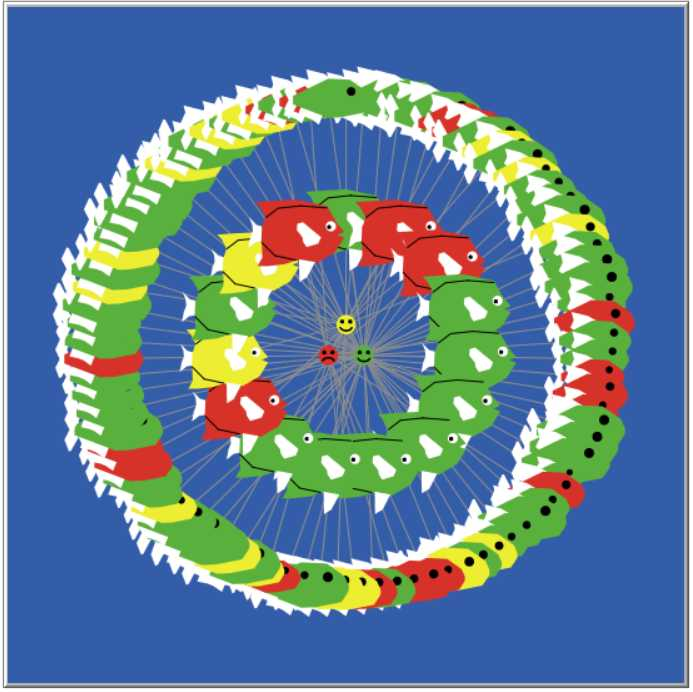
\includegraphics[width=.9\linewidth]{view} 

}

\caption{Investors are linked to Pools: a happy face represents a pool that has paid out, colours represent risk in a natural way (traffic lights), and the size of each fish correlates to the wealth of an investor.\label{fig:ui}}\label{fig:unnamed-chunk-1}
\end{figure}

\begin{figure}[p]

{\centering \includegraphics[width=.49\linewidth]{challenge_files/figure-latex/unnamed-chunk-2-1} \includegraphics[width=.49\linewidth]{challenge_files/figure-latex/unnamed-chunk-2-2} \includegraphics[width=.49\linewidth]{challenge_files/figure-latex/unnamed-chunk-2-3} 

}

\caption{\label{fig:plot_wealth0}Variation of Aggregate Wealth with number of coefficients and number of predictors, for $\tau=0$. Colour is used to distinguish one run for another, and has no other significance.}\label{fig:unnamed-chunk-2}
\end{figure}

\begin{figure}[p]

{\centering \includegraphics[width=.49\linewidth]{challenge_files/figure-latex/unnamed-chunk-3-1} \includegraphics[width=.49\linewidth]{challenge_files/figure-latex/unnamed-chunk-3-2} \includegraphics[width=.49\linewidth]{challenge_files/figure-latex/unnamed-chunk-3-3} 

}

\caption{\label{fig:plot_wealth1}Variation of Aggregate Wealth with number of coefficients with number of predictors, for $\tau=1$. Colour is used to distinguish one run for another, and has no other significance.}\label{fig:unnamed-chunk-3}
\end{figure}

\begin{figure}[p]

{\centering \includegraphics[width=.49\linewidth]{challenge_files/figure-latex/unnamed-chunk-4-1} \includegraphics[width=.49\linewidth]{challenge_files/figure-latex/unnamed-chunk-4-2} \includegraphics[width=.49\linewidth]{challenge_files/figure-latex/unnamed-chunk-4-3} 

}

\caption{\label{fig:plot_outgoings0}Variation of Payout per subscriber for $\tau=0$. NB: payout gradually stabilizes and tends to be confined to a narrow region that is better than break-even for subscribers.}\label{fig:unnamed-chunk-4}
\end{figure}

\begin{figure}[p]

{\centering \includegraphics[width=.49\linewidth]{challenge_files/figure-latex/unnamed-chunk-5-1} \includegraphics[width=.49\linewidth]{challenge_files/figure-latex/unnamed-chunk-5-2} \includegraphics[width=.49\linewidth]{challenge_files/figure-latex/unnamed-chunk-5-3} 

}

\caption{\label{fig:plot_outgoings1}Variation of Payout per subscriber , for $\tau=1$. NB: payout gradually stabilizes and tends to be confined to a narrow region that is better than break-even for subscribers.}\label{fig:unnamed-chunk-5}
\end{figure}

\begin{figure}[p]

{\centering \includegraphics[width=.49\linewidth]{challenge_files/figure-latex/unnamed-chunk-6-1} \includegraphics[width=.49\linewidth]{challenge_files/figure-latex/unnamed-chunk-6-2} \includegraphics[width=.49\linewidth]{challenge_files/figure-latex/unnamed-chunk-6-3} 

}

\caption{\label{fig:plot_sq0}Variation of Error for $\tau=0$. Colour is used to distinguish one run for another, and has no other significance.}\label{fig:unnamed-chunk-6}
\end{figure}

\begin{figure}[p]

{\centering \includegraphics[width=.49\linewidth]{challenge_files/figure-latex/unnamed-chunk-7-1} \includegraphics[width=.49\linewidth]{challenge_files/figure-latex/unnamed-chunk-7-2} \includegraphics[width=.49\linewidth]{challenge_files/figure-latex/unnamed-chunk-7-3} 

}

\caption{\label{fig:plot_sq1}Variation of Error for $\tau=1$. Colour is used to distinguish one run for another, and has no other significance.}\label{fig:unnamed-chunk-7}
\end{figure}

\begin{figure}[p]

{\centering \includegraphics[width=.49\linewidth]{challenge_files/figure-latex/unnamed-chunk-8-1} \includegraphics[width=.49\linewidth]{challenge_files/figure-latex/unnamed-chunk-8-2} \includegraphics[width=.49\linewidth]{challenge_files/figure-latex/unnamed-chunk-8-3} \includegraphics[width=.49\linewidth]{challenge_files/figure-latex/unnamed-chunk-8-4} 

}

\caption{\label{fig:plot_individual01}Growth of wealth for $\tau \in \{0,1\}$. Results are shown for a few of the richest individuals (judged at the end of the simulation), a few of the poorest, and a few in the middle. The figures on the left use linear predictors, those on the right are conservative.}\label{fig:unnamed-chunk-8}
\end{figure}

\begin{figure}[p]

{\centering \includegraphics[width=.49\linewidth]{challenge_files/figure-latex/unnamed-chunk-9-1} \includegraphics[width=.49\linewidth]{challenge_files/figure-latex/unnamed-chunk-9-2} \includegraphics[width=.49\linewidth]{challenge_files/figure-latex/unnamed-chunk-9-3} \includegraphics[width=.49\linewidth]{challenge_files/figure-latex/unnamed-chunk-9-4} 

}

\caption{\label{fig:plot_individual25}Growth of wealth for $\tau \in \{2,5\}$. The figures on the left use linear predictors, those on the right are conservative.}\label{fig:unnamed-chunk-9}
\end{figure}

\begin{figure}[p]

{\centering \includegraphics[width=.49\linewidth]{challenge_files/figure-latex/unnamed-chunk-10-1} \includegraphics[width=.49\linewidth]{challenge_files/figure-latex/unnamed-chunk-10-2} 

}

\caption{\label{fig:plot_individual_random}Growth of wealth for random assignments. Notice that some of the richest investors start lucky, and continue to be rich despite mediocre performance (the Trump effect).}\label{fig:unnamed-chunk-10}
\end{figure}

\begin{figure}[p]

{\centering 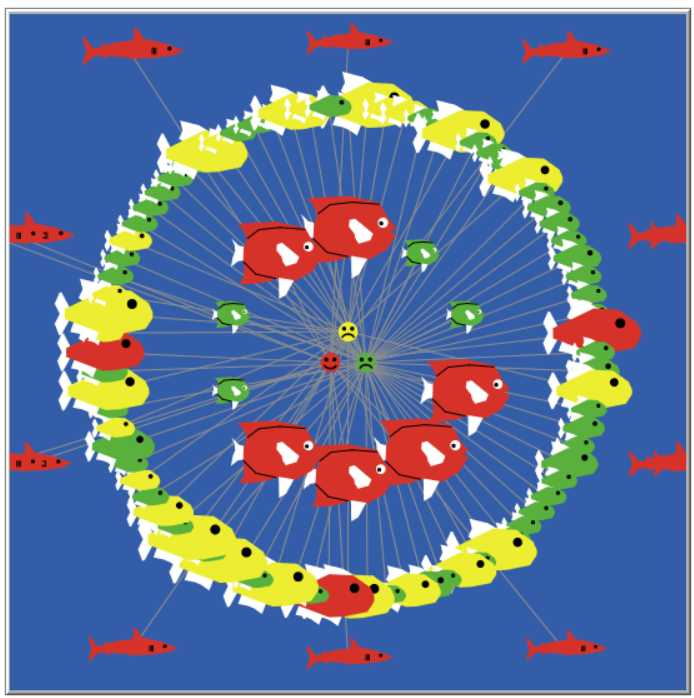
\includegraphics[width=.49\linewidth]{Cartel} 

}

\caption{Sharks represent members of the Cartel. It appears that cartel members are able to intimidate agents who use the first learning algorithm, but not the second.\label{fig:ui-cartel}}\label{fig:unnamed-chunk-11}
\end{figure}

\begin{figure}[p]

{\centering \includegraphics[width=.49\linewidth]{challenge_files/figure-latex/plot_cartel-1} 

}

\caption{\label{fig:cartel_return}Return from Cartel, compared with Stable Pool}\label{fig:plot_cartel}
\end{figure}

\begin{figure}[p]

{\centering \includegraphics[width=.49\linewidth]{challenge_files/figure-latex/plot_wealth-1} \includegraphics[width=.49\linewidth]{challenge_files/figure-latex/plot_wealth-2} 

}

\caption{\label{fig:tau_wealth}Variation of accumulated wealth with $\tau$}\label{fig:plot_wealth}
\end{figure}

\begin{figure}[p]

{\centering \includegraphics[width=.49\linewidth]{challenge_files/figure-latex/plot_errors-1} 

}

\caption{\label{fig:tau_error}Variation of Error with $\tau$}\label{fig:plot_errors}
\end{figure}

\begin{figure}[p]

{\centering \includegraphics[width=.49\linewidth]{challenge_files/figure-latex/plot_many_investors-1} \includegraphics[width=.49\linewidth]{challenge_files/figure-latex/plot_many_investors-2} \includegraphics[width=.49\linewidth]{challenge_files/figure-latex/plot_many_investors-3} \includegraphics[width=.49\linewidth]{challenge_files/figure-latex/plot_many_investors-4} 

}

\caption{\label{fig:many_investors}Many Investors, showing number in each pool. The reference line shows the maximum number of subscribers if pool is to be profitable.}\label{fig:plot_many_investors}
\end{figure}

\begin{figure}[p]

{\centering \includegraphics[width=.49\linewidth]{challenge_files/figure-latex/unnamed-chunk-12-1} \includegraphics[width=.49\linewidth]{challenge_files/figure-latex/unnamed-chunk-12-2} \includegraphics[width=.49\linewidth]{challenge_files/figure-latex/unnamed-chunk-12-3} \includegraphics[width=.49\linewidth]{challenge_files/figure-latex/unnamed-chunk-12-4} 

}

\caption{\label{fig:plot_individual_envy01}The effects of allowing agents to spy on each other--see Section \ref{heading:violate-sssumptions}. The top two plots form a control. The lower two show the effect of envy: if an agent is not in the upper stratum, as defined by the envy factor, it copies the behaviour of a randomly selected top player. See also remarks on Figure \ref{fig:plot_individual01}}\label{fig:unnamed-chunk-12}
\end{figure}

\begin{figure}[p]

{\centering \includegraphics[width=.49\linewidth]{challenge_files/figure-latex/unnamed-chunk-13-1} \includegraphics[width=.49\linewidth]{challenge_files/figure-latex/unnamed-chunk-13-2} \includegraphics[width=.49\linewidth]{challenge_files/figure-latex/unnamed-chunk-13-3} \includegraphics[width=.49\linewidth]{challenge_files/figure-latex/unnamed-chunk-13-4} 

}

\caption{\label{fig:plot_individual_envy23}The effects of allowing agents to spy on each other (continued).}\label{fig:unnamed-chunk-13}
\end{figure}

\begin{figure}[p]

{\centering \includegraphics[width=.49\linewidth]{challenge_files/figure-latex/unnamed-chunk-14-1} \includegraphics[width=.49\linewidth]{challenge_files/figure-latex/unnamed-chunk-14-2} \includegraphics[width=.49\linewidth]{challenge_files/figure-latex/unnamed-chunk-14-3} \includegraphics[width=.49\linewidth]{challenge_files/figure-latex/unnamed-chunk-14-4} 

}

\caption{\label{fig:plot_ergodic}Transient Behaviour. Plots show the number of steps required before the moving average over a few steps is close to the average over the entire run. We treat this as an estimate of the number of steps required for decay of the transient from starting conditions. NB: a value of 250 means that the trajectory has not stabilized, and is possibley chaotic: it does not mean that the trajectory has stabilized magically after 250 steps. }\label{fig:unnamed-chunk-14}
\end{figure}

\section*{References}\label{references}
\addcontentsline{toc}{section}{References}

\hypertarget{refs}{}
\hypertarget{ref-Challenge:2018}{}
{[}1{]} S. F. Institute, ``Spring 2018 complexity challenge.''
\url{https://www.complexityexplorer.org/challenges/2-spring-2018-complexity-challenge/submissions},
2018.

\hypertarget{ref-romero2014hedge}{}
{[}2{]} P. J. Romero and T. Balch, \emph{What hedge funds really do: An
introduction to portfolio management}. Business Expert Press, 2014.

\hypertarget{ref-arthur1994inductive}{}
{[}3{]} W. B. Arthur, ``Inductive reasoning and bounded rationality,''
\emph{The American economic review}, vol. 84, no. 2, pp. 406--411, 1994.

\hypertarget{ref-fogel1999inductive}{}
{[}4{]} D. B. Fogel, K. Chellapilla, and P. J. Angeline, ``Inductive
reasoning and bounded rationality reconsidered,'' \emph{IEEE
transactions on evolutionary computation}, vol. 3, no. 2, pp. 142--146,
1999.

\hypertarget{ref-challet1997emergence}{}
{[}5{]} D. Challet and Y.-C. Zhang, ``Emergence of cooperation and
organization in an evolutionary game,'' \emph{Physica A: Statistical
Mechanics and its Applications}, vol. 246, nos. 3-4, pp. 407--418, 1997.

\hypertarget{ref-Wilensky:1999}{}
{[}6{]} U. Wilensky, ``NetLogo,'' Center for Connected Learning;
Computer-Based Modeling, Northwestern University, Evanston, IL,
http://ccl.northwestern.edu/netlogo/, 1999 {[}Online{]}. Available:
\url{http://ccl.northwestern.edu/netlogo/}

\hypertarget{ref-Abelson:1985:SIC:26777}{}
{[}7{]} H. Abelson, G. J. Sussman, and J. Sussman, \emph{Structure and
interpretation of computer programs}. Cambridge, MA, USA: MIT Press,
1985.

\hypertarget{ref-wiki:closure}{}
{[}8{]} Wikipedia contributors, ``Closure (computer programming) ---
Wikipedia, the free
encyclopedia.''://en.wikipedia.org/w/index.php?title=Closure\_(computer\_programming)\&oldid=840549395,
2018.

\hypertarget{ref-rcore2018r}{}
{[}9{]} R Core Team, ``R: A language and environment for statistical
computing.'' R Foundation for Statistical Computing;
\url{https://www.R-project.org/}, Vienna, Austria, 2018.

\hypertarget{ref-allaire2018rmarkdown}{}
{[}10{]} J. Allaire \emph{et al.}, ``Rmarkdown: Dynamic documents for
r.'' \url{https://CRAN.R-project.org/package=rmarkdown}, 2018.

\hypertarget{ref-vanhespen2016thesis}{}
{[}11{]} R. van Hespen, ``Writing your thesis with r markdown (2) --
text, citations and equations.''
\url{https://rosannavanhespenresearch.wordpress.com/2016/02/17/writing-your-thesis-with-rmarkdown-2-making-a-chapter/},
2016.

\hypertarget{ref-wiki:roshambo}{}
{[}12{]} Wikipedia contributors, ``Rock--paper--scissors --- Wikipedia,
the free encyclopedia.''
\url{https://en.wikipedia.org/w/index.php?title=Rock\%E2\%80\%93paper\%E2\%80\%93scissors\&oldid=841658701},
2018.

\hypertarget{ref-hill2009knowing}{}
{[}13{]} T. P. Hill, ``Knowing when to stop,'' \emph{American
scientist}, vol. 97, no. 2, pp. 126--133, 2009.


\end{document}
